\section{The loss-function Migdal probability}\label{sec:12.3}

A dark-matter particle of \SI{300}{MeV} can give a silicon nucleus a momentum of \SI{1.6}{MeV} and a recoil energy of \SI{47}{eV}. The momentum is seven hundred times the size of the Brillouin zone, the recoil energy a thousand times that of a phonon, and the nucleus leaves its site as a free particle (\cref{sec:11.4}). The electrons it sets in motion take a momentum of a few keV, and half of the time they receive less than \SI{4.6}{eV}, a few times the gap. In this regime the Migdal entry \cref{eq:12.1-Skk} of the joint response simplifies twice. The lattice factor collapses to a free recoil, and the electronic factor becomes the loss function $L(\vect{p},\omega_e)$ that \cref{sec:10.2} used for the electron-recoil rate. The probability that a kick leaves an electron--hole pair is then fixed by one material function, an integral of $L$ over momenta weighted by $\omega_e^{-4}$, and it comes out thirty times larger in crystalline silicon than in a silicon atom. The same function sets the rate per unit target mass, which \cref{sec:17.5} uses to compare materials.

\subsection{Migdal probability through the loss function}\label{sec:12.3-soft}

Three approximations take \cref{eq:12.1-Skk} to the loss function: the diagonal $\vect{G} = \vect{G}'$ of the electronic factor, a free recoil, and the soft limit $p \ll q$. On the diagonal the integral over the zone and the sum over $\vect{G}$ then combine into one integral over the unreduced momentum $\vect{p} = \vect{k} + \vect{G}$ given to the electrons. By \cref{eq:4.4-SL}, with the diagonal inverse dielectric matrix \cref{eq:E.6-L}, the diagonal element of the density response at $\vect{p}$ is the loss function at that momentum:
\begin{equation}
  S^{ee}_{\vect{G}\vect{G}}(\vect{k},\omega_e) = \frac{2p^2}{e^2}\,L(\vect{p},\omega_e) , \qquad \omega_e > 0,\; T \ll \Eg .
  \label{eq:12.3-See}
\end{equation}
The local fields on the diagonal stay inside $L$; the dropped elements $\vect{G} \ne \vect{G}'$ carry the part of the local fields that couples different momenta, and we return to both parts of the local fields below. The free recoil treats each nucleus as if it were alone and in the impulse regime, so that the lattice factor is the free recoil of \cref{sec:11.4} at the momentum $\vect{q} - \vect{p}$ the nucleus keeps, $S^{\mathrm{ad}}_{\kappa}(\vect{q} - \vect{p},\omega_l) = 2\pi\nd_\kappa\,\delta(\omega_l - |\vect{q} - \vect{p}|^2/2M_\kappa)$. The \emph{soft limit} $p \ll q$ says that the electrons take a small part of the momentum. The lattice factor then becomes $2\pi\nd_\kappa\,\delta(\omega_l - E_R)$ with $E_R = q^2/2M_\kappa$, and it no longer depends on $\vect{p}$. The Migdal entry then factorizes into the free recoil and a probability per kick,
\begin{equation}
  S_{\kappa\kappa}(\vect{q};\omega_l,\omega_e) = 2\pi\nd_\kappa\,\delta(\omega_l - E_R)\,\frac{\dd P_{\mathrm{Mig}}}{\dd\omega_e} .
  \label{eq:12.3-factor}
\end{equation}

The vertex is the potential of the moving ion. In silicon the ten electrons of the $1s$, $2s$ and $2p$ shells are bound by \SI{100}{eV} or more and follow their nucleus; for the valence electrons whose response is $L$, nucleus and core act together as one ion. The potential of this ion is
\begin{equation}
  v_\kappa(\vect{p}) = -\frac{Z_{\mathrm{ion}}(p)\,e^2}{p^2} , \qquad Z_{\mathrm{ion}}(p) = Z_\kappa - f^{\mathrm{core}}_\kappa(p) ,
  \label{eq:12.3-Zion}
\end{equation}
with $f^{\mathrm{core}}_\kappa(p)$ the form factor of the core electrons, the Fourier transform of their density. \Cref{eq:12.3-Zion} defines the \emph{valence ionization factor} $Z_{\mathrm{ion}}(p)$. At small $p$ it is the ionic charge, 4 for silicon; at large $p$ the probe resolves the core and $Z_{\mathrm{ion}}$ rises toward the nuclear charge 14. With the core orbitals of the free atom from \cref{sec:3.5}, $Z_{\mathrm{ion}}$ of silicon exceeds 4 by \SI{5}{\percent} at \SI{2.4}{keV} and by \SI{10}{\percent} at \SI{3.4}{keV}, and reaches 4.84 at \SI{5}{keV} and 6.78 at \SI{10}{keV}. The split between core and valence is a convention, and $Z_{\mathrm{ion}}$ must count exactly the electrons that $L$ leaves out.

When \cref{eq:12.3-See,eq:12.3-Zion} and the lattice factor are inserted in \cref{eq:12.1-Skk}, the factors combine as
\begin{equation*}
  \frac{1}{2\pi}\,\frac{(\vect{q}\cdot\vect{p})^2}{M_\kappa^2\omega_e^4}\,\frac{Z_{\mathrm{ion}}^2e^4}{p^4}\,\frac{2p^2}{e^2}\,L\;2\pi\nd_\kappa
  = 2\pi\nd_\kappa\,\frac{e^2}{\pi}\,\frac{Z_{\mathrm{ion}}^2(\vect{v}_N\cdot\vect{p})^2}{\omega_e^4\,p^2}\,L ,
\end{equation*}
with $\vect{v}_N = \vect{q}/M_\kappa$ the recoil velocity of \cref{sec:6.1}. Since $e^2/\pi = 4\alpha$, comparison with \cref{eq:12.3-factor} gives the result.
\begin{keyresult}[The crystal Migdal probability in the soft limit]
For a kick of momentum $\vect{q}$ in the impulse regime, with $p \ll q$, the probability per unit electronic energy that a nucleus of species $\kappa$ leaves the valence electrons excited is
\begin{equation}
  \frac{\dd P_{\mathrm{Mig}}}{\dd\omega_e} = 4\alpha\int\frac{\dd^3p}{(2\pi)^3}\;Z_{\mathrm{ion}}(p)^2\,\frac{(\vect{v}_N\cdot\vect{p})^2}{\omega_e^4\,p^2}\,L(\vect{p},\omega_e)
  = \frac{4\alpha v_N^2}{3\,\omega_e^4}\,L_{\mathrm{Mig}}(\omega_e) ,
  \label{eq:12.3-soft}
\end{equation}
where the second form holds for a direction-averaged loss function and defines the Migdal-weighted loss function
\begin{equation}
  L_{\mathrm{Mig}}(\omega_e) = \int\frac{\dd^3p}{(2\pi)^3}\;Z_{\mathrm{ion}}(p)^2\,\bar L(p,\omega_e) .
  \label{eq:12.3-LMig}
\end{equation}
\end{keyresult}
\noindent This is the formula of Knapen, Kozaczuk and Lin~\cite[Eq.~(6)]{knapen2021migdal}. Read as a product, it is the probability of a dipole boost, $v_N^2$, times the response of the electrons to the field of a charge $Z_{\mathrm{ion}}$ that has suddenly started to move. The screening and the local fields of \cref{sec:10.2} enter here unchanged. The factor $\omega_e^{-4}$ is the square of the boost denominator $\omega_e^2$ of \cref{eq:12.1-amp}. With $v_N^2 = 2E_R/M_\kappa$ the probability grows linearly with the recoil energy, and the material enters only through $L_{\mathrm{Mig}}$.

For silicon we evaluate \cref{eq:12.3-soft} with the loss function of Knapen, Kozaczuk and Lin with local fields~\cite{knapen2021dark}, which is the table of \cref{sec:10.2}. We count the table from \SI{1.11}{eV}, the step-model gap that accompanies it, rather than from its scissor gap, the physical \SI{1.17}{eV}; the table stops at \SI{89}{eV} and \SI{22.5}{keV}. At $E_R = \SI{100}{eV}$, reached at $q = \SI{2.29}{MeV}$ with $v_N = 8.74\times10^{-5}$ (\SI{26}{km/s}), the probability is $P_{\mathrm{Mig}} = 6.1\times10^{-3}$, or $6.1\times10^{-5}$ per eV of recoil energy. Half of the probability lies below $\omega_e = \SI{4.6}{eV}$ and \SI{89}{\percent} below \SI{10}{eV}; the mean is \SI{6.0}{eV}. The momenta are larger than the zone: the median $p$ is \SI{5.7}{keV}, two and a half times $q_{\mathrm{BZ}}$ of \cref{eq:11.1-qBZ}, and \SI{97}{\percent} of the probability comes from $p > q_{\mathrm{BZ}}$. The plasmon, at $p \lesssim \SI{2.5}{keV}$, carries \SI{4}{\percent}: the factor $\omega_e^{-4}$ favors the single-pair continuum near the gap over the plasmon at \SI{17}{eV}. With a point ion of charge 4 instead of $Z_{\mathrm{ion}}(p)$ the probability falls to $3.9\times10^{-3}$, lower by a factor 1.57.

\begin{workedexample}{The coefficient $4\alpha$ from the f-sum}\label{we:12-fsum}
The coefficient of \cref{eq:12.3-soft} can be checked without the diagrams of \cref{eq:12.1-Skk}, from a sum rule. Take one Fourier component $\vect{p}$ of the force of the ion, $F_{\vect{p}} = \vect{v}_N\cdot\nabla_{\vect{X}}V_{eN}$ restricted to that component. By \cref{eq:12.1-force} it is $-\ii(\vect{v}_N\cdot\vect{p})\,v_\kappa(\vect{p})\,n_e(\vect{p})/\Vol$ up to a phase, and the Migdal amplitude to a final state $j$ is $\langle\Psi_j|F_{\vect{p}}|\Psi_0\rangle/\Delta E_j^2$. The fifth moment of the probability weighs each final state with $\Delta E_j^5$ and therefore equals the energy-weighted sum $\sum_j\Delta E_j|\langle\Psi_j|F_{\vect{p}}|\Psi_0\rangle|^2$. For the density operator this sum is the f-sum rule \cref{eq:4.3-fsum}, $\sum_j\Delta E_j|\langle\Psi_j|n_e(\vect{p})|\Psi_0\rangle|^2 = N_ep^2/2m_e$ at $T = 0$, which holds for the interacting electrons exactly. Per unit volume the fifth moment is therefore
\begin{equation*}
  (\vect{v}_N\cdot\vect{p})^2\,|v_\kappa(\vect{p})|^2\,\frac{\nd_e\,p^2}{2m_e} = (\vect{v}_N\cdot\vect{p})^2\,\frac{Z_{\mathrm{ion}}^2e^4}{p^4}\,\frac{\nd_e\,p^2}{2m_e} .
\end{equation*}
The loss-function form with an unknown coefficient $c$ in place of $4\alpha$ gives instead, with the f-sum of the loss function $\int_0^\infty\dd\omega\,\omega L = (\pi/2)\omega_p^2$ (\cref{eq:10.2-moments}) and $\omega_p^2 = e^2\nd_e/m_e$,
\begin{equation*}
  c\,Z_{\mathrm{ion}}^2\,\frac{(\vect{v}_N\cdot\vect{p})^2}{p^2}\int_0^\infty\dd\omega\,\omega L = c\,Z_{\mathrm{ion}}^2\,\frac{(\vect{v}_N\cdot\vect{p})^2}{p^2}\,\frac{\pi}{2}\,\frac{e^2\nd_e}{m_e} .
\end{equation*}
The two fifth moments agree if $c = e^2/\pi = 4\alpha$, at every $\vect{p}$ and for any electron density.

For silicon the check also measures the table. At the valence density, $\nd_e = \SI{2.00e23}{cm^{-3}}$ and $\omega_p^{\mathrm{val}} = \SI{16.6}{eV}$, the table holds 0.94, 0.93, 0.92 and 0.90 of the f-sum at $p = 1$, 2, 3 and \SI{5}{keV}, so the fifth moment of the computed spectrum is within \SI{10}{\percent} of its exact value there. At \SI{7.5}{keV} the table holds 0.62 and at \SI{10}{keV} only 0.17, because the free-electron peak $p^2/2m_e$ moves past the table's last energy of \SI{89}{eV}. The probability is far less sensitive than the fifth moment, since $\omega_e^{-4}$ weights the low energies the table does contain. The momenta above \SI{10}{keV} give \SI{2.3}{\percent} of $P_{\mathrm{Mig}}$, and an upper bound on the energies beyond the table follows from the same sum rule, $\int_{\omega_{\mathrm{top}}}^\infty\dd\omega\,L/\omega^4 \le (\pi/2)\omega_p^2/\omega_{\mathrm{top}}^5$. At $\omega_{\mathrm{top}} = \SI{89}{eV}$, summed over the momenta of the table, the bound is \SI{1.6}{\percent} of the probability below $\omega_{\mathrm{top}}$.
\end{workedexample}

The material input of \cref{eq:12.3-soft} is the loss function of the valence electrons at momenta up to about \SI{20}{keV}, where the Migdal weight ends, and energies from the gap to about \SI{50}{eV}. At these momenta the calculation needs the diagonal elements far from the head; \cref{sec:10.2} met the same requirement for electron recoil. An all-electron calculation of $L$ at $p \le \SI{30}{keV}$ removes the need for $Z_{\mathrm{ion}}$ and puts the core shells in the same table. The random-phase loss function does not contain the Migdal lines of excitons below the gap.

\subsection{Validity of the soft limit}\label{sec:12.3-validity}

Knapen and collaborators state \cref{eq:12.3-soft} with the scalar dielectric function $\varepsilon(\vect{p},\omega)$ and note that it holds only for $\vect{p}$ in the first zone~\cite[text after Eq.~(6)]{knapen2021migdal}. Inside the zone the scalar function is the macroscopic one, and the loss function is the head of the inverse matrix. Outside it, a scalar function of $|\vect{p}|$ has no unique meaning, and the derivation above says which element to take: the diagonal element of the inverse at the reciprocal vector that contains $\vect{p}$. The distinction matters because the Migdal weight lies outside the zone. \Cref{lim:12.3a} compares, momentum by momentum, the loss function that a scalar random-phase $\varepsilon$ gives with the diagonal element of the inverse with local fields. The two agree within \SI{10}{\percent} up to $p = 1.3\,q_{\mathrm{BZ}} = \SI{2.9}{keV}$, which holds \SI{8}{\percent} of the probability. Beyond, the scalar function overestimates the weight by \SI{24}{\percent} at $2q_{\mathrm{BZ}}$ and \SI{35}{\percent} at $3q_{\mathrm{BZ}}$, where the probability peaks, and the total by a factor 1.35. The mechanism is the one of \cref{sec:10.2}: at $|\vect{p}| \approx 2$--$3\,|\vect{G}_{111}|$ the charge induced in the cell has a macroscopic component that screens the field of the ion.
\begin{limitbox}[Crystal Migdal effect through the loss function][lim:12.3a]
$\dd P/\dd\omega = 4\alpha\int\dd^3p/(2\pi)^3\,Z_{\mathrm{ion}}(p)^2|\vect{v}_N\cdot\vect{p}|^2\,\Imag[-1/\varepsilon(\vect{p},\omega)]/(\omega^4p^2)$ with a scalar dielectric function, for $\vect{p}$ in the first zone~\cite[Eq.~(6)]{knapen2021migdal}.
\par\smallskip
{\centering
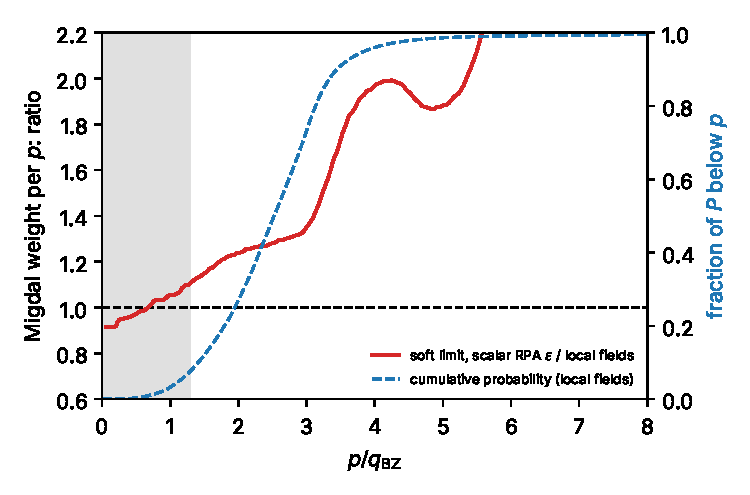
\includegraphics[width=\linewidth]{figures/ch12/limit12_3a.pdf}
\captionof{figure}{Migdal weight of silicon per unit momentum $p$ given to the electrons, $p^2Z_{\mathrm{ion}}(p)^2\int_{\Eg}\dd\omega\,L(p,\omega)/\omega^4$, from the loss function of a scalar random-phase dielectric function at $|\vect{p}|$ (no local fields), divided by the same with the diagonal element of the inverse dielectric matrix with local fields, against $p/q_{\mathrm{BZ}}$ ($q_{\mathrm{BZ}} = \SI{2.25}{keV}$). Both from the direction-averaged tables of Knapen, Kozaczuk and Lin~\cite{knapen2021dark} (threshold \SI{1.11}{eV}, the step-model gap that accompanies them, $\omega \le \SI{89}{eV}$), smoothed over \SI{0.7}{keV} in $p$; $Z_{\mathrm{ion}}(p)$ of \cref{eq:12.3-Zion}. The elements $\vect{G} \neq \vect{G}'$ are in neither curve. Dashed, right axis: the fraction of $P_{\mathrm{Mig}}$ carried by momenta below $p$. Gray band: $p \le 1.3\,q_{\mathrm{BZ}}$, where the two agree within \SI{10}{\percent}; it holds \SI{8}{\percent} of the probability.}\label{fig:12-limit-3a}
\par}
\smallskip
Beyond the first zone the scalar form has to be replaced by the diagonal of the inverse dielectric matrix, and the local fields lower the silicon probability by a factor 1.35; the elements $\vect{G} \neq \vect{G}'$ are the next correction.
\end{limitbox}

The elements $\vect{G} \neq \vect{G}'$ keep the full matrix in \cref{eq:12.1-Skk}. For a direction-averaged target the boost factor averages to $\langle[\hat{\vect{q}}\cdot(\vect{k}+\vect{G})][\hat{\vect{q}}\cdot(\vect{k}+\vect{G}')]\rangle = (\vect{k}+\vect{G})\cdot(\vect{k}+\vect{G}')/3$. At the random-phase level the response matrix is $S^{ee}_{\vect{G}\vect{G}'} = (2|\vect{k}+\vect{G}||\vect{k}+\vect{G}'|/e^2)\,\Imag[-(\tilde\varepsilon^{-1})_{\vect{G}\vect{G}'}]$, with the symmetrized matrix $\tilde\varepsilon_{\vect{G}\vect{G}'} = \delta_{\vect{G}\vect{G}'} - v_{\mathrm{C}}^{1/2}(\vect{k}+\vect{G})\,R^0_{\vect{G}\vect{G}'}(\vect{k},\omega)\,v_{\mathrm{C}}^{1/2}(\vect{k}+\vect{G}')$, which has the same inverse diagonal as $\varepsilon$. In a crystal with time reversal and inversion it is symmetric, $\tilde\varepsilon_{\vect{G}\vect{G}'} = \tilde\varepsilon_{\vect{G}'\vect{G}}$, but not Hermitian at frequencies where the crystal absorbs; $\Imag[-(\tilde\varepsilon^{-1})_{\vect{G}\vect{G}'}]$ denotes the anti-Hermitian part $[(\tilde\varepsilon^{-1})^\dagger - \tilde\varepsilon^{-1}]_{\vect{G}\vect{G}'}/2\ii$, which for a symmetric matrix is the imaginary part element by element. With a constant ion charge, $L_{\mathrm{Mig}}$ of \cref{eq:12.3-LMig} becomes
\begin{equation}
  \begin{aligned}
  L_{\mathrm{Mig}}(\omega) &= \frac{Z_{\mathrm{ion}}^2}{\Omega}\,\mathcal{F}_{\mathrm{Mig}}(\omega) , \\
  \mathcal{F}_{\mathrm{Mig}}(\omega) &= \sum_{\vect{G}\vect{G}'}\int_{\mathrm{BZ}}\frac{\Omega\,\dd^3k}{(2\pi)^3}\,\frac{(\vect{k}+\vect{G})\cdot(\vect{k}+\vect{G}')}{|\vect{k}+\vect{G}|\,|\vect{k}+\vect{G}'|}\,\ee^{\ii(\vect{G}-\vect{G}')\cdot\vect{\tau}_\kappa}\,\Imag\bigl[-(\tilde\varepsilon^{-1})_{\vect{G}\vect{G}'}(\vect{k},\omega)\bigr] ,
  \end{aligned}
  \label{eq:12.3-FL}
\end{equation}
where $\vect{\tau}_\kappa$ is the position of the struck nucleus in the cell, averaged over the equivalent sites of its species. The indices are in the order of $S^{ee}_{\vect{G}\vect{G}'}$ in \cref{eq:12.1-Skk}, with $n_e(\vect{k}+\vect{G})^\dagger$ on the left of $R^0_{\vect{G}\vect{G}'}$; the transposed order reverses the sign of the phase. The reversal leaves silicon unchanged, since its two sites are images under inversion, but not GaAs. The phase belongs to the struck nucleus: the off-diagonal elements depend on where the origin of $\varepsilon$ is placed, and the phase is one only when the origin sits on that atom. The diagonal terms carry no phase and give back \cref{eq:12.3-LMig} at any origin. The off-diagonal terms need the full matrix, which the tables of \cref{sec:10.2} do not contain. In an empirical-pseudopotential random-phase model of silicon, with the phase of \cref{eq:12.3-FL}, the full matrix exceeds the diagonal form on the total by a factor of 1.38 with $8^3$ points $\vect{k}$ and $|\vect{G}|^2 \le 19\,(2\pi/a)^2$ and of about 1.2 when extrapolated in both. The two numbers are not a bracket: the factor still falls as reciprocal-lattice vectors are added, and the fall is not slowing, so 1.2 is not a lower bound. The off-diagonal elements raise the rate at every truncation computed, and the factor is flat in $\mchi$. The model carries only about two thirds of the diagonal local-field effect of \cref{lim:12.3a}, so its off-diagonal size is a guide, not a bound in either direction. The full local-field calculation that would replace the model estimate is open.

The free recoil is the second approximation. Below the impulse onset of \cref{sec:11.4}, $x_R = 4$ at $q = \SI{92.5}{keV}$ in silicon, the lattice takes the recoil as single phonons and multiphonons, not as a free particle. In the soft limit, however, the lattice factor drops out of the probability. It enters the rate only through the energy balance $\omega = \omega_e + \omega_l$ in $\vmin$, and the lattice energy has the mean $E_R$ in every regime (\cref{eq:5.6-sum}) and is small against $\omega_e$: \SI{0.16}{eV} at the onset, against a few eV. Replacing the free recoil by the incoherent response of a bound silicon nucleus at all phonon orders, including its zero-phonon line, changes the rate by less than $10^{-5}$ at every mass from 3 to \SI{110}{MeV} (\cref{lim:12.3b}). The impulse onset is therefore not where the Migdal formula fails.

Dropping $\vect{p}$ from the lattice factor, the soft limit as defined above, leaves the electronic spectrum unchanged, because the lattice factor has unit weight at every $\vect{q} - \vect{p}$ (\cref{sec:12.4}). The boost amplitude remains to be examined, and it expands in $v_Np/\omega_e$, not in $p/q$. For a free nucleus the kick and the Coulomb exchange with the electrons come in two time orderings~\cite[Eq.~(1)]{liang2021describing}. Kicked first, the nucleus moves with $\vect{q}$, passes $\vect{p}$ to the electrons and leaves with $\vect{q} - \vect{p}$; the energy denominator is $\omega_e - b + a$, with $b = \vect{q}\cdot\vect{p}/M_\kappa$ and $a = p^2/2M_\kappa$. With the exchange first, the nucleus recoils with $-\vect{p}$ before the kick, and the denominator is $\omega_e + a$. The boost factor $(\vect{v}_N\cdot\vect{p})/\omega_e^2$ becomes
\begin{equation}
  \frac{1}{\omega_e - b + a} - \frac{1}{\omega_e + a} = \frac{b}{(\omega_e - b + a)(\omega_e + a)} = \frac{b}{\omega_e^2}\Bigl(1 + \frac{b - 2a}{\omega_e} + \cdots\Bigr) ,
  \label{eq:12.3-bracket}
\end{equation}
the free-nucleus case of \cref{eq:12.4-exact}. The numerator of \cref{eq:12.3-bracket} is $\vect{q}\cdot\vect{p}/M_\kappa$ at every $p$: the velocity in the boost is that of the kicked nucleus, whatever momentum the electrons take. Averaged over the angle $c$ between $\vect{q}$ and $\vect{p}$, the square gives
\begin{equation*}
  \Bigl\langle\frac{b^2}{(\omega_e - b + a)^2(\omega_e + a)^2}\Bigr\rangle = \frac{v_N^2p^2}{3\omega_e^4}\Bigl[1 - \frac{2p^2}{M_\kappa\omega_e} + \frac95\,\frac{v_N^2p^2}{\omega_e^2} + \cdots\Bigr] ,
\end{equation*}
the free-nucleus part of \cref{eq:12.4-corr}. The terms odd in $c$ drop out; in a crystal they drop out because the loss function is even under $\vect{p} \to -\vect{p}$ in any target with time reversal. There is no term in $p/q$, so the soft limit does not fail when the electrons take a momentum comparable with the kick. The recoil term $2p^2/M_\kappa\omega_e$ is $2\times10^{-3}$ at the median $p$ near the gap. The Doppler term $\tfrac95v_N^2p^2/\omega_e^2$ grows with the recoil energy; it is the shift $\vect{v}_N\cdot\vect{p}$ of the electronic energy by the moving nucleus, taken at second order. Weighted with the silicon spectrum, the Doppler term is 0.04 at $E_R = \SI{100}{eV}$, 0.13 at \SI{300}{eV} and 0.42 at \SI{1}{keV}. It is only the leading term. Near the gap $v_Np/\omega_e$ is already 0.41 at the median $p$ and $E_R = \SI{100}{eV}$, and the higher orders of \cref{eq:12.3-bracket} add as much again. With the exact bracket the soft-limit probability is low by the factor 0.93 at \SI{100}{eV}, 0.79 at \SI{300}{eV} and 0.62 at \SI{500}{eV}, whereas the leading term alone gives 0.96, 0.90 and 0.85. The soft limit holds within \SI{10}{\percent} up to $E_R \approx \SI{160}{eV}$, the spectrum-weighted counterpart of the bound $v_Np/\omega_e \le 0.27$ found near the gap at fixed $p$ in \cref{lim:12.4a}. Toward \SI{1}{keV} the expansion breaks down. There $v_Np$ at the median momentum is \SI{1.6}{eV}, above the gap, and the denominator $\omega_e - b + a$ vanishes inside the range of the integral: the kicked nucleus, already moving, ionizes the electrons as a slow ion does. Ionization by the already moving nucleus is an on-shell two-step process, the electronic stopping of the recoiling ion, not a Migdal transition, and the second-order amplitude does not describe it. The momenta where the denominator vanishes hold \SI{0.9}{\percent} of the soft-limit probability at \SI{500}{eV} and \SI{3.7}{\percent} at \SI{1}{keV}.
\begin{limitbox}[Crystal Migdal rate with free recoil][lim:12.3b]
$\mathcal{R} = (\rho_\chi/\mchi)\,[2A^2\sigma_p\,Z_{\mathrm{ion}}^2\,\alpha N_T/(3\mu_{\chi n}^2\Omega M^2)]\int\dd^3v\,(f/v)\int p_N^3\,\dd p_N\int\dd\omega\,\omega^{-4}\,\Theta(v - \vmin)\,\mathcal{F}_{\mathrm{Mig}}(\omega)$, $\vmin = p_N/2\mu_{\chi N} + \omega/p_N$, with $N_T$ the number of nuclei per unit target mass, $\Omega$ the cell volume, $p_N$ the momentum transfer, the soft-limit amplitude and $\mathcal{F}_{\mathrm{Mig}}$ of \cref{eq:12.3-FL}~\cite[Eqs.~(1), (7), (11), (12)]{liang2021describing}.
\par\smallskip
{\centering
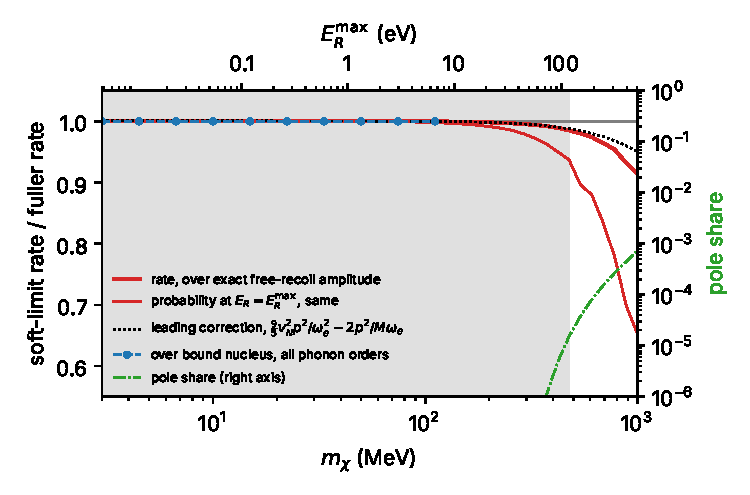
\includegraphics[width=\linewidth]{figures/ch12/limit12_3b.pdf}
\captionof{figure}{Total Migdal rate of silicon ($\omega_e \ge \SI{1.11}{eV}$, heavy mediator) in the soft limit with a free recoil, divided by two fuller results, against the dark-matter mass; top axis, the largest recoil energy $E_R^{\max} = 2\mu_{\chi N}^2v_{\mathrm{max}}^2/M$. Thick solid: over the rate with the exact free-recoil amplitude \cref{eq:12.3-bracket}. Thin solid: the same ratio for the probability at $E_R = E_R^{\max}$, the end of the recoil spectrum. Dotted: the leading correction $\frac95v_N^2p^2/\omega_e^2 - 2p^2/M_\kappa\omega_e$ alone. Dashed with points: over the soft-limit rate with the incoherent response of a bound nucleus at all phonon orders and $T = 0$ (density of states of \cref{sec:5.2}); it differs from one by less than $10^{-5}$. Dash-dotted, right axis: the share of the soft-limit rate at momenta where the exact amplitude has a pole, $v_Np \ge \omega_e + p^2/2M_\kappa$, which both rates of the ratio leave out. Every curve uses the same diagonal loss function with local fields and $Z_{\mathrm{ion}}(p)$ in place of $\mathcal{F}_{\mathrm{Mig}}$, and the halo of \cref{sec:1.2}. Gray band: $\mchi \lesssim \SI{0.5}{GeV}$, where the probability at the end of the recoil spectrum is within \SI{10}{\percent} of the exact one.}\label{fig:12-limit-3b}
\par}
\smallskip
Above about \SI{0.5}{GeV} the end of the recoil spectrum passes $E_R \approx \SI{160}{eV}$, where the motion of the nucleus during the electronic transition changes the probability by more than \SI{10}{\percent}, and near \SI{1}{keV} the moving nucleus ionizes the electrons by itself; the binding of the nucleus changes the soft-limit rate by less than $10^{-5}$ at every mass from 3 to \SI{110}{MeV}.
\end{limitbox}

\noindent From 3 to \SI{150}{MeV} the soft-limit rate is within $1.1\times10^{-3}$ of the exact free-recoil rate, and at \SI{1}{GeV}, where the rate integrates over the whole recoil spectrum, it is low by the factor 0.91.

Below the onset the bound amplitude of \cref{sec:12.4} stays within a few parts in $10^3$ of the soft limit (\cref{eq:12.4-corr}). At low mass, therefore, neither the soft limit nor the lattice limits the formula; the electronic factor does (\cref{lim:12.3a}).

The core shells stay frozen in $Z_{\mathrm{ion}}$. Their own excitation is a separate Migdal process of atomic type, with the boost of each core shell (\cref{sec:12.2}). The $2p$ shell of an isolated silicon atom gives $7.1\times10^{-5}$ at $E_R = \SI{100}{eV}$, \SI{1.2}{\percent} of the valence probability, at $\omega_e$ above \SI{100}{eV}. And the formula needs no restriction to $\mchi \ll M_\kappa$: the reduced mass $\mu_{\chi N}$ in $\vmin$ keeps the recoil of a heavy particle, and only the per-mass form below drops it.

\subsection{Crystal and atomic spectra of silicon}\label{sec:12.3-atom}

The crystal formula and the atomic formula of \cref{sec:12.2} answer the same question for the same nucleus, and they differ by more than an order of magnitude. \Cref{fig:12-crystal-atom} shows both at $E_R = \SI{100}{eV}$. The crystal probability is $6.1\times10^{-3}$. The isolated silicon atom, with all its shells and the Dirac--Hartree--Fock tables of Cox and collaborators~\cite{cox2023precise}, gives $2.1\times10^{-4}$, of which $1.3\times10^{-4}$ come from the $3s$ and $3p$ valence shells. The crystal is 29 times the whole atom and 47 times its valence shells.

\begin{figure}[tbp]
  \centering
  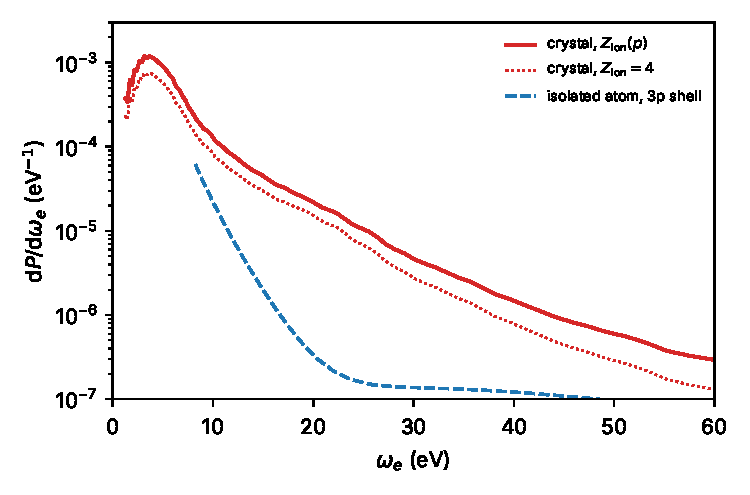
\includegraphics[width=0.75\linewidth]{figures/ch12/fig12_3.pdf}
  \caption{Migdal ionization spectra of silicon at the recoil energy $E_R = \SI{100}{eV}$ ($v_N = 8.74\times10^{-5}$), against the energy $\omega_e$ given to the electrons. Solid: the crystal, \cref{eq:12.3-soft}, with the loss function of Knapen, Kozaczuk and Lin with local fields (diagonal, direction-averaged, threshold \SI{1.11}{eV}, the step-model gap that accompanies the tables) and $Z_{\mathrm{ion}}(p)$ of \cref{eq:12.3-Zion}; $P_{\mathrm{Mig}} = 6.1\times10^{-3}$. Dotted: the same with a point ion, $Z_{\mathrm{ion}} = 4$; $3.9\times10^{-3}$. Dashed: the $3p$ shell of an isolated atom at dipole order, from the Dirac--Hartree--Fock tables of Cox, Dolan, McCabe and Quiney~\cite{cox2023precise} rescaled by $v_N^2$, with $\omega_e$ the kinetic energy of the electron plus the measured ionization energy of the atom, \SI{8.15}{eV}; $1.2\times10^{-4}$. The atomic $3s$ ($1.0\times10^{-5}$) and the core shells ($8\times10^{-5}$, nearly all $2p$ above \SI{100}{eV}) are not drawn.}
  \label{fig:12-crystal-atom}
\end{figure}

The ratio of the crystal to the atomic probability can be read off the figure. The crystal threshold is lower: the crystal spectrum starts at the gap, \SI{1.1}{eV}, the atomic one at the ionization energy of \SI{8.15}{eV}, and with the weight $\omega_e^{-4}$ the region between the two thresholds holds \SI{84}{\percent} of the crystal probability. Above \SI{8}{eV} the crystal is still larger, six times at \SI{10}{eV} and sixty times at \SI{20}{eV}. There the crystal spectrum acts as a loss function, which concentrates the oscillator strength of the valence electrons in the plasmon and the broad interband peak around it, between 10 and \SI{25}{eV}; the atom has only the tail of its $3p$ continuum there. The vertex differs too. The atom is boosted with all its electrons, and the boost probes each orbital at the momentum $q_e = m_ev_N$, \SI{45}{eV} at $E_R = \SI{100}{eV}$, far below the inverse size of any shell. The crystal formula probes the valence electrons at the momenta $p$ of the ion's field, mostly 3 to \SI{9}{keV}, where $Z_{\mathrm{ion}}(p)$ adds the factor 1.6 of the point-ion comparison.

None of the three differences makes the atom a lower bound on the crystal in general. A crystal with a gap larger than the ionization energy of its atoms would not show the first difference, and one with valence electrons as localized as atomic ones would not show the second.

\subsection{The Migdal rate per unit mass}\label{sec:12.3-rate}

The rate follows from the free-recoil spectrum \cref{eq:11.4-LS} by weighting each recoil with its Migdal probability. A recoil of momentum $q$ that also gives the electrons $\omega_e$ needs the minimum speed \cref{eq:1.3-vmin} at $\omega = \omega_e + q^2/2M_\kappa$, which is $\vmin = \omega_e/q + q/2\mu_{\chi N}$. With $\dd E_R = q\,\dd q/M_\kappa$ and \cref{eq:12.3-soft}, the rate per unit target mass of a crystal of one species, for a heavy mediator, is
\begin{equation}
  \begin{aligned}
  \frac{\dd\mathcal{R}}{\dd\omega_e} &= \frac{\rho_\chi\,\sigma_N}{2\mchi\,\mu_{\chi N}^2M_\kappa}\int\dd q\;q\,\eta\Bigl(\frac{\omega_e}{q} + \frac{q}{2\mu_{\chi N}}\Bigr)\frac{\dd P_{\mathrm{Mig}}}{\dd\omega_e} \\
  &= \frac{2\alpha\,\rho_\chi\,\sigma_N}{3\mchi\,\mu_{\chi N}^2M_\kappa^3}\,\frac{L_{\mathrm{Mig}}(\omega_e)}{\omega_e^4}\int\dd q\;q^3\,\eta\Bigl(\frac{\omega_e}{q} + \frac{q}{2\mu_{\chi N}}\Bigr) .
  \end{aligned}
  \label{eq:12.3-rate}
\end{equation}
For a compound each species adds its term with $1/M_\kappa$ replaced by its number of nuclei per unit mass. \Cref{eq:12.3-rate} is the formula of \cref{lim:12.3b} with $\mathcal{F}_{\mathrm{Mig}}$ replaced by its diagonal.

When $\omega_e$ is small against the kinetic energy of the dark matter, it can be dropped from $\vmin$, and the momentum integral becomes a moment of the halo: with $u = q/2\mu_{\chi N}$, $\int\dd q\,q^3\eta(q/2\mu_{\chi N}) = 16\mu_{\chi N}^4\int_0^\infty\dd u\,u^3\eta(u) = 4\mu_{\chi N}^4\langle v^3\rangle$, since $\int_0^\infty\dd u\,u^3\eta(u) = \int\dd^3v\,f_\chi(\vect{v})\,v^3/4$. For the halo of \cref{sec:1.2}, $\langle v^3\rangle^{1/3} = \SI{401}{km/s}$. With $\sigma_N = A^2\sigma_p\mu_{\chi N}^2/\mu_{\chi n}^2$ and $A_\kappa/M_\kappa = 1/m_u$, a compound of $N_\kappa$ atoms of each species per formula unit, of mass number $A_{\mathrm{cell}} = \sum_\kappa N_\kappa A_\kappa$, gives
\begin{equation}
  \frac{\dd\mathcal{R}}{\dd\omega_e} = \underbrace{\frac{8\alpha\,\rho_\chi\,\sigma_p\,\langle v^3\rangle}{3\,m_u^3}\,\frac{\mu_{\chi N}^4}{\mchi\,\mu_{\chi n}^2}}_{\text{halo and coupling}}\;\underbrace{\frac{1}{\omega_e^4}\sum_\kappa\frac{N_\kappa\,L_{\mathrm{Mig},\kappa}(\omega_e)}{A_{\mathrm{cell}}}}_{\text{material}} ,
  \label{eq:12.3-permass}
\end{equation}
where $L_{\mathrm{Mig},\kappa}$ is \cref{eq:12.3-LMig} with the ion factor of species $\kappa$, and $\mu_{\chi N}$ is taken equal for all species, as it is for $\mchi \ll M_\kappa$. This is the factorized rate of Knapen and collaborators~\cite[Eqs.~(1), (6) and (A36)]{knapen2021migdal} in per-mass form. The mass dependence $\mu_{\chi N}^4/(\mchi\mu_{\chi n}^2)$ grows as $\mchi$ below the nucleon mass and as $\mchi^3$ between the nucleon and the nuclear mass. This factor has the local exponents 1.01 between 5 and \SI{10}{MeV}, 1.24 between 100 and \SI{200}{MeV}, and 2.07 between 3 and \SI{6}{GeV}, where $\mu_{\chi N}$ already falls below $\mchi$. The material enters as $L_{\mathrm{Mig}}$ per nucleon: at fixed $L_{\mathrm{Mig}}$ the nuclear mass drops out, so that light nuclei win only if their ions keep a comparable $L_{\mathrm{Mig}}$, and comparing materials means comparing loss functions weighted by $Z_{\mathrm{ion}}^2$ and $\omega_e^{-4}$.

The comparison of materials carries a convention: $Z_{\mathrm{ion}}$ must count the electrons that are not in the loss function. For nickel the small-$p$ ion charge is 2, 10 or 18 according as $L$ holds the $4s$ electrons, the $3d$ and $4s$, or also the $3s$ and $3p$; the choice changes the nickel term by a factor 25 to 81. And the weight $\omega_e^{-4}$ makes $L_{\mathrm{Mig}}/\omega_e^4$ dominated by the region just above the gap: for a loss function that starts at $\Eg$, the f-sum bounds $\int\dd\omega\,L/\omega^4$ by $(\pi/2)\omega_p^2/\Eg^5$ at each $p$, so that a small gap is worth more than a large oscillator strength. \Cref{sec:17.5} uses \cref{eq:12.3-permass} as the Migdal figure of merit.

\begin{limitbox}[Per-mass Migdal rate with the valence ionization factor][lim:12.3c]
$\dd\mathcal{R}/\dd\omega \propto \mu_{\chi N}^4\mchi^{-1}\mu_{\chi n}^{-2}\,\omega^{-4}\sum_\kappa N_\kappa L_{\mathrm{Mig},\kappa}(\omega)/A_{\mathrm{cell}}$, the factorized soft-limit rate with free-recoil kinematics in which $\omega$ is dropped from energy conservation~\cite[Eqs.~(1), (6)]{knapen2021migdal}.
\par\smallskip
{\centering
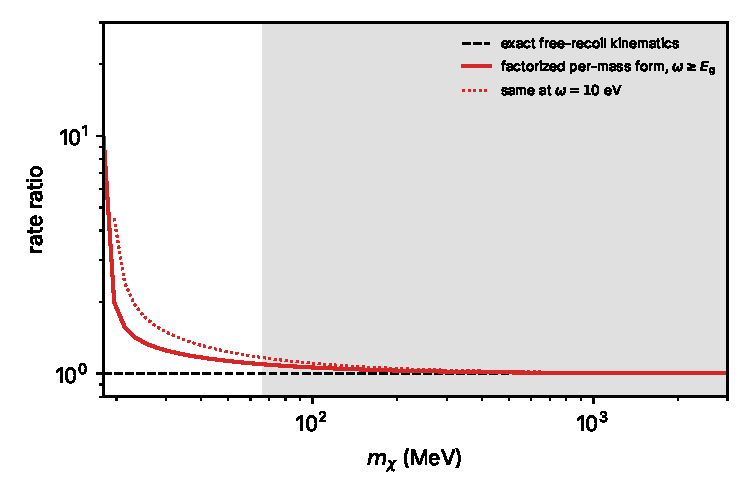
\includegraphics[width=\linewidth]{figures/ch12/limit12_3c.pdf}
\captionof{figure}{Migdal rate of silicon from the per-mass form \cref{eq:12.3-permass}, divided by the rate \cref{eq:12.3-rate} with the exact free-recoil kinematics, against the dark-matter mass. Solid: total rate for $\omega_e \ge \SI{1.11}{eV}$; dotted: the spectrum at $\omega_e = \SI{10}{eV}$. Both rates: heavy mediator, $\sigma_p = 10^{-38}\,\mathrm{cm}^2$, halo of \cref{sec:1.2}, the loss function with local fields and $Z_{\mathrm{ion}}(p)$, and momentum transfers above the impulse onset $q \ge \SI{92.5}{keV}$. Gray band: $\mchi \ge \SI{66}{MeV}$, where the total is within \SI{10}{\percent}.}\label{fig:12-limit-3c}
\par}
\smallskip
Below about \SI{60}{MeV} the electronic energy is no longer small against the kinetic energy of the dark matter. The per-mass form then overestimates the rate, by a factor 1.25 at \SI{30}{MeV} and 1.85 at \SI{20}{MeV}, and the exact $\vmin$ of \cref{eq:12.3-rate} must be kept.
\end{limitbox}

For orientation, at $\sigma_p = 10^{-38}\,\mathrm{cm}^2$ the exact rate \cref{eq:12.3-rate} above the onset is 1.9 events per kg and year at \SI{30}{MeV}, 30 at \SI{100}{MeV} and 970 at \SI{1}{GeV}. These are rates of primary pairs of a few eV, with the spectrum of \cref{fig:12-crystal-atom}. The number of electrons a detector counts follows from the cascade of \cref{chap:18}.
